
\section{モデルと標本の乖離による過誤}
データとモデルを統計量により比較したとき、その乖離について測ることのできないことをまとめる。

\subsection{モデルの確率密度関数と標本の分布の乖離による過誤}
経験がないことで、適当なモデルを構築し、非常に少数のサンプルサイズしか得られないことで、そのモデルの妥当性について検証できないまま、モデルとデータを仮説検定により比較し、判断することにより生じる間違いである。
例えば、データの分布が非対称に分布しているのに、正規分布を含んだ統計モデルを構築し、$T$統計量により検定をおこなったとする\footnote{データが非対称に分布していることから、正規分布を含んだ統計モデルでは推論できないことがわかるので、統計検定を使う意義はなくなると思う}。前の節でみたように、分布関数に対して適切な統計量を選ばなければ$\alpha_1$が設定した有意水準$\alpha$とならないので、期待していた推論が行えないことが多くなる。

\subsection{無作為抽出されていない事による過誤}
対象を無作為に抽出できていない標本から、統計量を計算し、モデルの母数を推定したとする。
このモデルでは、本来設定した母集団に関する予測には誤りが多くなる。
例えば、17歳の日本人男性の身長を母集団に指定したのに、17歳のバスケ部部員の身長を計測すると、その標本はひどく偏ったものになる。
その標本を元に、モデルの母数を推定し、母集団に関する推測を行う。
すると、間違った推測が得られる。例えば、平均が大きくなりすぎたりすることが予想される。

\subsubsection{後付けの母集団かつ$p<\alpha$を満たす集団}
母集団Aを設定し、標本を抽出したものを標本aとする。標本aのデータはさまざまな要素から構成されているとする。例えば、ある会社に所属する人の、身長や年収、税金の支払い履歴、ローン残高、労働部署、高校時代の部活などであるとする。
この標本から、何らかの属性$A'$に当てはまるデータbを抽出したとする。
データbについて特定の統計モデルとの乖離するかを調べ、乖離していることをが判明したとする(乖離を定量的に調べる方法はなんでもいいが、$p<\alpha$だったと考えても良い)。
この結果から、属性$A'$に関わると考えられる母集団A'を再構成する。
そこから、母集団$A'$を特定のモデルで予測できないと結論づけることはできない。
図\ref{fig:conceptual_diagram_HARKing}}には、概念図を示しておいた。

まず、今集めた標本$a$は、母集団$A$から集めたものであり、母集団$A'$から集めたものではない。
よって、母集団$A'$から無作為抽出できていない。
また、標本aを無作為抽出したときに付随して得た、母集団$A'$の一部のデータである。
以上から、母集団$A'$に関するデータとモデルの乖離を検証することができてない。


\subsubsection{後付けの母集団かつ$p<\alpha$を満たす集団}
$p<\alpha$であるという標本がデータから発見されたので、標本の特性を持つと思われる母集団を後付けし、その母集団から無作為抽出を行なったことにし、統計モデルが棄却されたというストーリーを作ったとする。
言い換えれば、後付けの母集団ならば、$p<\alpha$であるという論理を構築したことになる。
実際には、後付けの母集団でありかつ$p<\alpha$という集団から作為抽出しているので\footnote{この場合でも無作為抽出できていると誤解してしまうが、後付けの母集団から無作為抽出できていない!}、本来の母集団については何もわからない。言い換えれば、母集団に関する拡大解釈が行われたことで、母集団に関しては何もわからないのに、推測を行なったと間違えた主張をしている\footnote{実際調査した母集団に対して報告した母集団デカすぎんだろ...}。
母集団の特徴を知るには、無作為抽出を行い、推測を行う必要がある。


\begin{figure}
    \begin{center}
        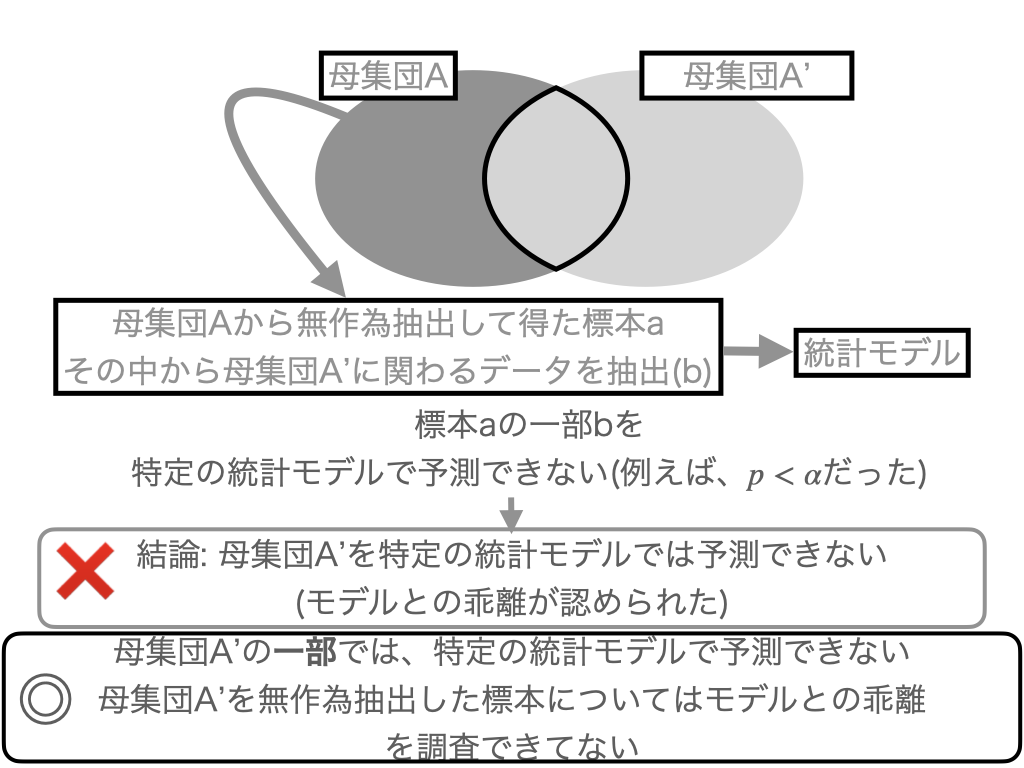
\includegraphics[width=15cm]{./image/01_/conceptual_diagram/conceptual_diagram.005.png}
        \caption{仮説ハッキングの概念図}
        \label{fig:conceptual_diagram_HARKing}
    \end{center}
\end{figure}
    

このような母集団に関する拡大解釈を仮説ハッキング($HARKing$(Hypothesizing After the Results are Known))といい、この操作により得たデータと仮説について、仮説が元からあったことにして、報告を行うと、研究不正となる\footnote{
    HARKingは、再現性の問題という意見もある。
    \url{https://twitter.com/ykamit/status/1077716200845500416} 。この意見に私は同意する。私は、母集団を無作為抽出していないことで、再現できないことが増えると考えられる。
}
\footnote{
    多重検定により、$p$値が低く推測されることが問題であるというものもある\cite{池田_功毅2016,中村_大輝2021sp20016}。部分的には同意できるが、私は十分理解できなかった。
}\footnote{
    Twitterでのアンケートでは、多くの人がHARkingをうまく理解できてないというTwitterでのアンケートもある。
    \url{https://twitter.com/biomedcircus/status/1088957697368690689}
}\footnote{
    探索的なデータ解析においては、帰無仮説の後付けが許されるという主張もある。この意見には同意できない。母集団について拡大解釈をすることは許されない。探索的データ解析により得られるのは、母集団かつ$p<\alpha$という集団が見つかったということのみ主張でき、母集団についての推測をしたと主張はしない方が良い。
}\footnote{
    HARKingについては、\cite{kerr1998harking}に詳しくまとめられている
}。



\begin{SMbox}{HARKing}
    \begin{rightbubbles}{bubblegreen}{Yuki Kamitani}{./image/Twitter_logo_EPS/2021_Twitter_logo_blue.eps}
    データを操作してp値をいじる行為を不正と認識している人は多いが、HARKingが不正と思っている人は非常に少ない。私の周辺分野のシニア研究者で理解している人はほぼ皆無(問題を指摘すると一笑に付される)。研究の実践と論文フォーマットの齟齬やフェアプレー精神の問題(?)と理解している人がいた
        \begin{flushright} 
            \small	\url{https://twitter.com/ykamit/status/1077715969827528705}
        \end{flushright}    
    \end{rightbubbles}
  \end{SMbox}
  

\subsubsection{$p<\alpha$になったら無作為抽出を終える}
$p$値がある値を下回ったときに、実験を終了するという操作を行なったとする。
統計モデルの予測と一致するように、母集団を選択したことになる。
この場合、無作為抽出した集団により、設定した母集団に関する性質を調べるという研究目的を達成できない。
「母集団かつ設定したモデルにおいて$p<\alpha$である」集団に関する調査を行なっていることになる。

調査を終えて、この標本についてモデルを使った予測ができないと主張できない。
この不正な操作をアステリスクシーキングという。

\if 0
\subsection{標本の分布がわからない事による過誤}
TODO: よくわからない。
以上により仮説検定は、既知の母集団と変異を与えた母集団との違いを図る方法の一つの方法であると言える。
母集団分布が既知でないならば統計モデルをかんで構築する必要があり、そこから変異を捉えることを試みると、
モデルの仮定と標本の特徴が一致しないことにより、過誤が生じる。

\subsubsection{独立同分布ではない事による過誤}
モデルでは、確率変数は独立であるが、自然現象の多くはなんらかの相関を持っていることが多い。
人間の身長であっても、同じ社会の中にいれば、各個人がなんからの相関を持つとも考えられる。
そんなことは、おいておいて、それぞれ独立だと思って解析してみると言うのが統計学を使った方法であるので、
自然とモデルの間にはやはりギャップが存在し、モデルの想定よりもあらい推定になることがあり得る。
\fi
\if 0
\paragraph{$p<0.05$にした理由}
https://biolab.sakura.ne.jp/statistics-5-percent.html
\fi



\if 0
\subsection{サンプルサイズが小さければ$t$検定}
西内啓 著「統計学が最強の学問である(実践編)」(ダイヤモンド社)
\url{https://biolab.sakura.ne.jp/small-sample-t-test-glm.html}
\fi 
